The experiment from which the unknown parameter values are derived employs bioengineered micropatterning techniques. The micropatterns form a regular arrangement of circular 2D ‘patches’ populated with cells surrounded by an exposed substrate. The exposed regions emulate necrotic areas of the retinal tissue that result from repeated exposure to reactive oxidative species, triggering neovascularization and exudative AMD \cite{Chopdar2003Age}. Recreating these regular spatially organized cellular configurations is essential to understanding the impact of local cell-cell and cell-environment interactions on VEGF autoregulation. 

In the experimental study, described in \cite{qanitabaker:Vargis2014Effect}, the bioengineered circular micro patterns were employed to control the extent of cell-cell interactions, which occur within the patch, and cell-environment interactions, which occur at the perimeter. Several patch sizes were used in this study ( \SI{100}{\micro\metre}, \SI{200}{\micro\metre}, \SI{300}{\micro\metre}, and \SI{400}{\micro\metre}) to sample the proportion of cell-cell and cell-environment interactions in each experiment. Such sampling constrains the possible parameter values. Each patch was seeded with retinal pigment epithelial (RPE) cells and grown in a cellular culture. As the cells grew, the VEGF per cell was measured at regular intervals: 4, 24, 30 48, 54, 72 hours. To measure the VEGF per cell, enzyme-linked immunosorbent assay (ELISA) was used to determine the total VEGF contained within the cell culture, and the number of cells per patch was determined by image analysis proceeded by staining. Figure~\ref{in_vitro_experiment}(a) (taken from \cite{qanitabaker:Vargis2014Effect}) illustrates the stained patches at 72 hours. Experiments were repeated ten times and averaged. The final spatiotemporal data produced is illustrated in Figure~\ref{in_vitro_experiment}(b) and forms the target prediction for the computational model simulation.

The bioengineered experiments were simulated using a hybrid agent-based approach, which is an extension of \textsl{iDynoMiCs} framework developed by the Kreft group at University of Birmingham \cite{qanitabaker:Lardon2011IDynoMiCS}. This model was selected because of its extensibility and easy of use. All inputs to the model such as parameter values and initial condition are easily specified using an XML document called the protocol file. Hybrid models integrate discrete components to represent the cells and continuous equations to represent biochemical reactions and diffusion. Each cell is a spherical particle that grows by consuming nutrient and accumulating biomass volume; when the volume exceeds twice the initial volume, cell division is simulated by splitting the particle into two. Particles can secrete and uptake soluble biochemicals (such as VEGF) which diffuse through the domain; regulatory reactions that model interactions among intracellular and inter-cellular proteins become PDEs. The simulation interlaces cellular growth and movement (implemented by relaxing forces between particles) with biochemical redistribution (implemented by solving the PDEs). Random noise disrupts cellular movement and the division volume to represent the inherent stochasticity of the biological processes.

The setup of the simulations replicate the experimental conditions and units of the \textit{in vitro} experiments. The 2D domain size of each simulation is \SI{2400}{\micro\metre} by \SI{2400}{\micro\metre}, initial cell size is set to $80 \mu m^2$ and the doubling time due to growth is set at 36 hours. Each simulation begins with multiple RPE cells distributed randomly at the same density and with the patch pattern. The simulation replicates the first 72 hours of the \textit{in vitro} experiments. Illustrations of the simulated experiments are shown in Figure~\ref{simulation_examples}.

This framework is inherently multiscale in that the parameters that control the low-level mechanisms at the cellular level, e.g., growth, the VEGF secretion rate and autoregulation, determine the cell population and VEGF concentration over the complete multicellular domain. Figure~\ref{simulation_examples} illustrate the VEGF distributions in the domain. To compute the VEGF concentration per cell, the total VEGF is computed over the whole domain, while the number of cells is directly determined by the simulator. This approach intrinsically includes the quantitative spatiotemporal control effects as the cells grow, secret VEGF which diffuses over the domain. Moreover, the simulations provide insight into the spatial VEGF gradients within and between patches, unavailable in \textit{in vitro} studies.

%\cite{qanitabaker:Cao2007Spatiotemporal}

% \begin{figure}[!t]
%  \centering
%
% \begin{subfigure}{.5\textwidth}
%   \centering
%   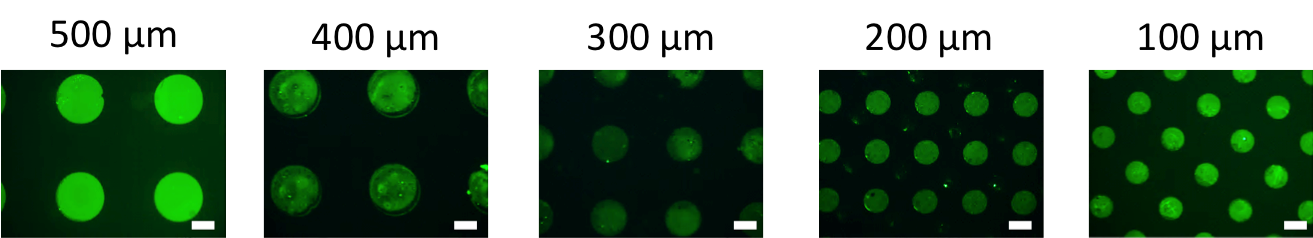
\includegraphics[width=.8\linewidth]{./figures/in_vitro_crop.png}
%   \caption{(a) Patches of stained RPE cells at 72 hours for each patch size. \cite{qanitabaker:Vargis2014Effect}.}
%
% \end{subfigure}%
%
% \begin{subfigure}{.5\textwidth}
%   \centering
%   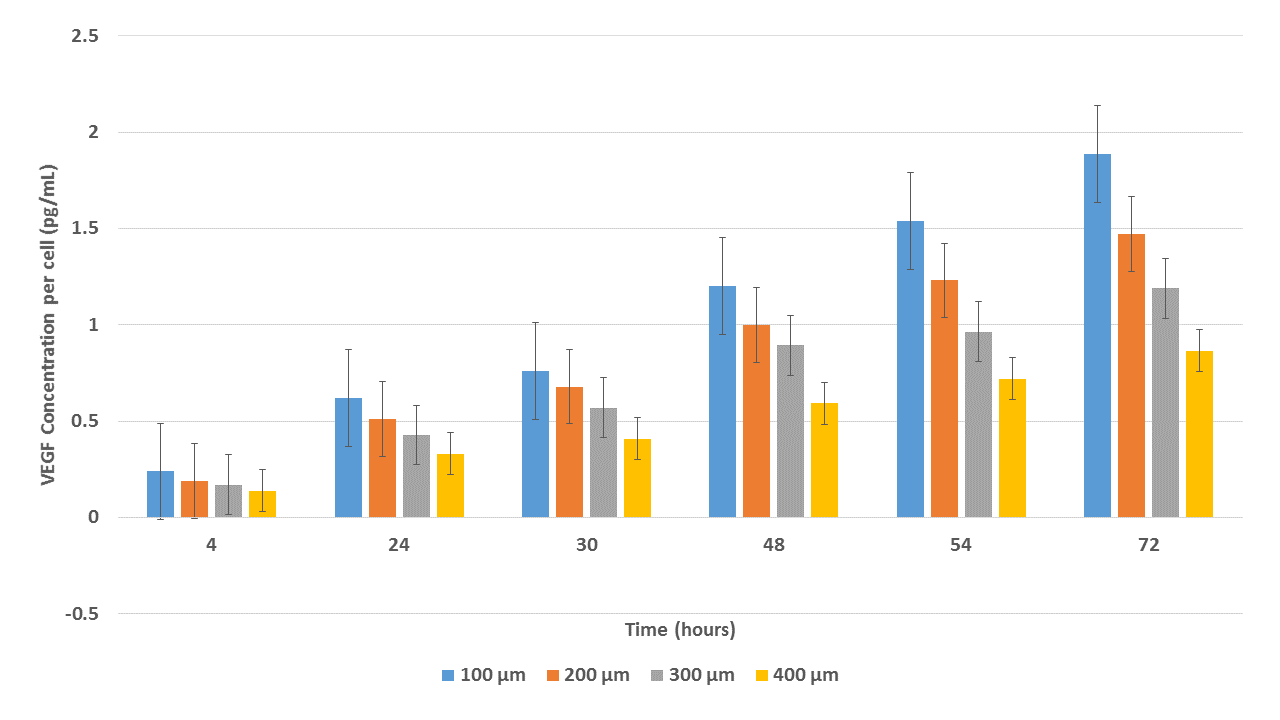
\includegraphics[width=.8\linewidth]{./figures/Results/In-Vitro.png}
%   \caption{(b) Time course of VEGF expression per cell measured at 4, 24, 30, 48, and 72 h ( data for each time from the \textit{in vitro} \cite{qanitabaker:Vargis2014Effect} ).}
% \end{subfigure}%
%\label{in_vitro_experiment}
%\end{figure}







\begin{figure}
 \begin{center}
  \begin{tabular}{cc}
   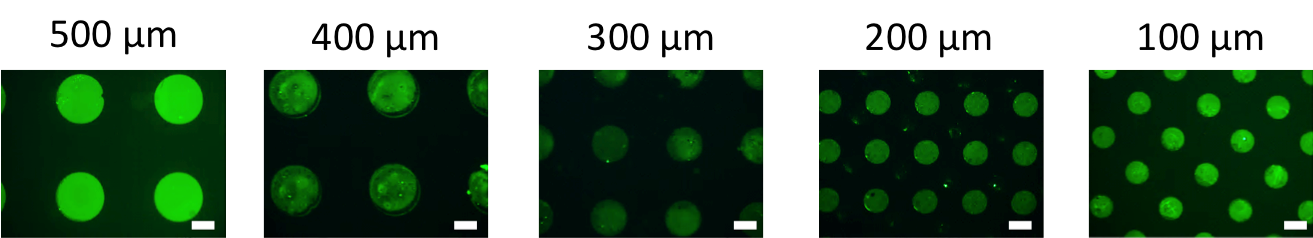
\includegraphics[width=0.40\textwidth]{./figures/in_vitro_crop.png} \\
   (a)\\
    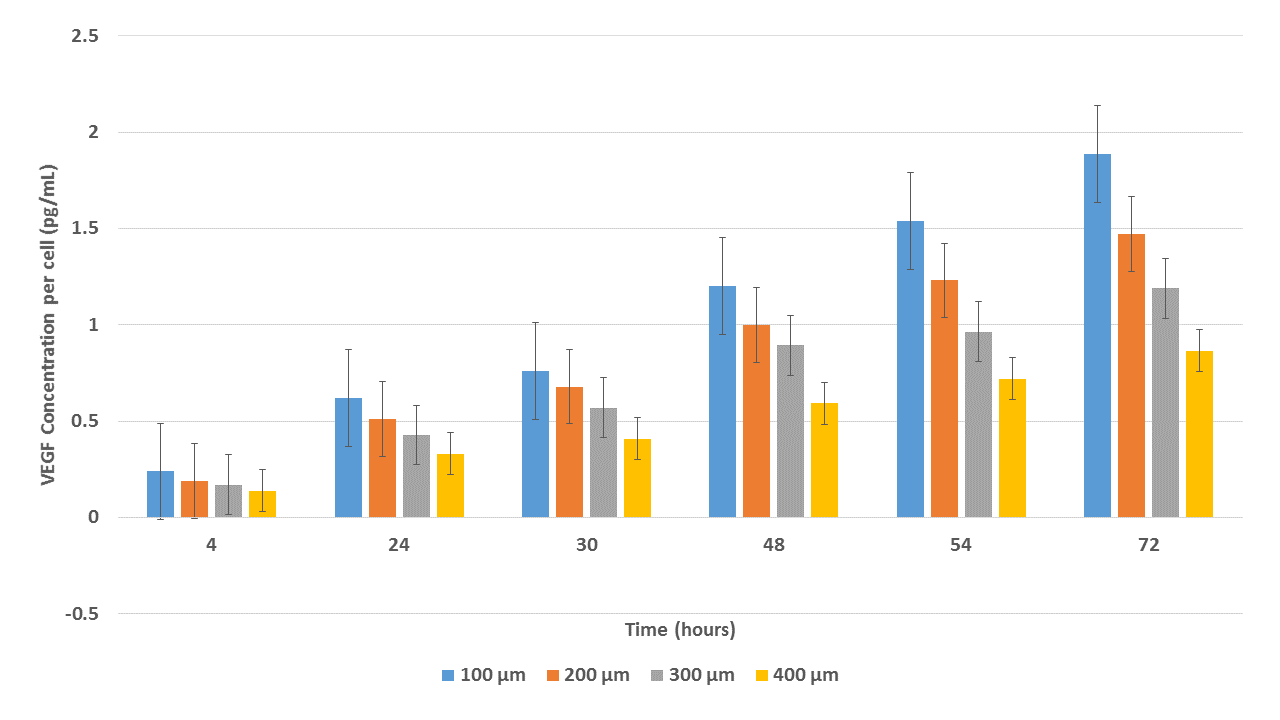
\includegraphics[width=0.40\textwidth]{./figures/Results/In-Vitro.png} \\
   (b)   
   \end{tabular}
   \end{center}

\caption{(a) Patches of stained RPE cells at 72 hours for each patch size. \cite{qanitabaker:Vargis2014Effect}. (b) Time course of VEGF expression per cell measured at 4, 24, 30, 48, and 72 h ( data for each time from the \textit{in vitro} \cite{qanitabaker:Vargis2014Effect} ). }
  \vspace{+1mm}
\label{in_vitro_experiment}
\end{figure}


 The autoregulation of VEGF secretion is described in Equation~\ref{VEGF_autoregulation} as a function of biomass $M$ and local VEGF concentration $V$. The diffusion coefficient of VEGF, $D_{V}$, is set to $5.8 \times 10^{-11} m^{2} s^{-1}$ given in microfluidic experiments from \cite{qanitabaker:Shin2012Microfluidic}.

 \begin{equation}
 \frac{\partial V}{\partial t}=D_{V}\bigtriangledown^{2} V+ \mu _{V}  \frac{K}{ \beta V+K} M
 \label{VEGF_autoregulation}
 \end{equation}

Over time, the RPE cells grow based on a doubling time of 36 hours \cite{qanitabaker:Bryckaert2000Regulation}, which determines the growth rate parameter $\mu _{M}$. Since nutrient is unlimited and cell crowding is not an issue within the 72 hour time line, we applied first order kinetics for cell growth as shown in Equation \ref{Cell_Growth}.\\


\begin{equation}
\frac{\partial M}{\partial t}=   \mu _{M} M
\label{Cell_Growth}
\end{equation}

Table \ref{parameters} summarizes the description of the parameters used in the equations above and identifies the known parameters and those that need to be determined by the method introduced in this paper.

\begin{table}[ht]
\caption{ Known and unknown parameter descriptions} % title of Table
\centering
\begin{footnotesize}
\begin{tabular}{l l l}
\hline
Parameter   &  Value & Description\\ \hline \hline
%\\ [1ex]      % [1ex] adds vertical space
$D_{V}$     & $5.8 \times 10^{-11} m^{2} s^{-1}$ & Diffusion coefficient \\
$\mu _{M}$  &  1.0194   $ hour^{-1}$                 & Max. growth rate for RPE cells \\
[1ex]      % [1ex] adds vertical space
\hline
%\\ [1ex]      % [1ex] adds vertical space
$K$       &  \textsl{Unknown}                  & Auto regulation rate \\
$\mu _{V}$ & \textsl{Unknown}                   & Secretion rate \\
$\beta $    &  \textsl{Unknown}                  & Binding affinity \\
[1ex]      % [1ex] adds vertical space
 

 
 
\hline
\end{tabular}
\end{footnotesize}
\label{parameters}
\end{table}

\begin{figure}
 \begin{center}
  \begin{tabular}{cc}
   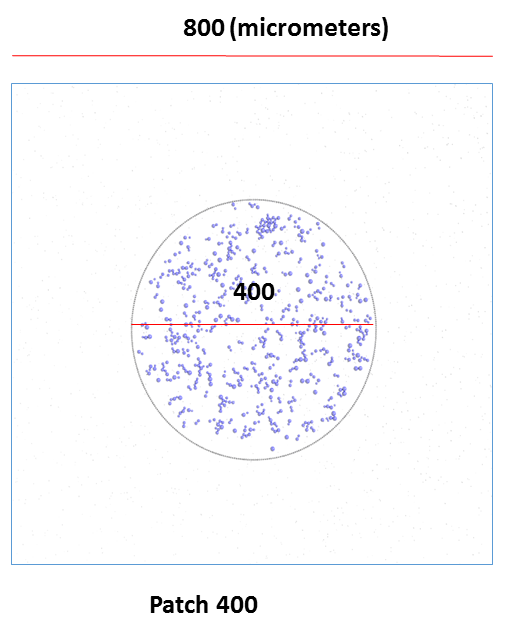
\includegraphics[width=0.20\textwidth]{./figures/400_one.png} &   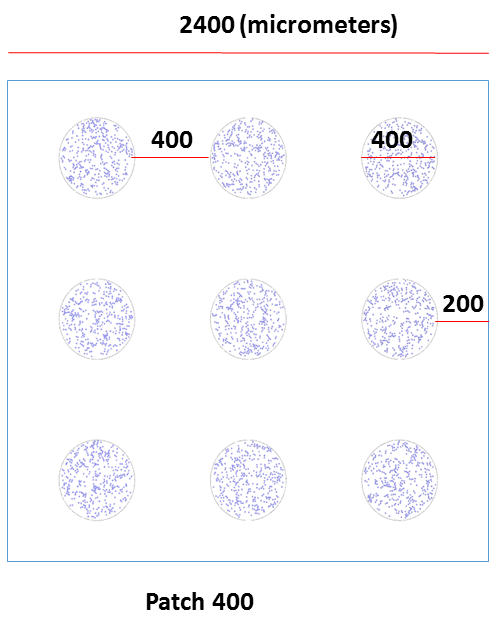
\includegraphics[width=0.20\textwidth]{./figures/Patch400.png} \\
   (a) & (b) \\
   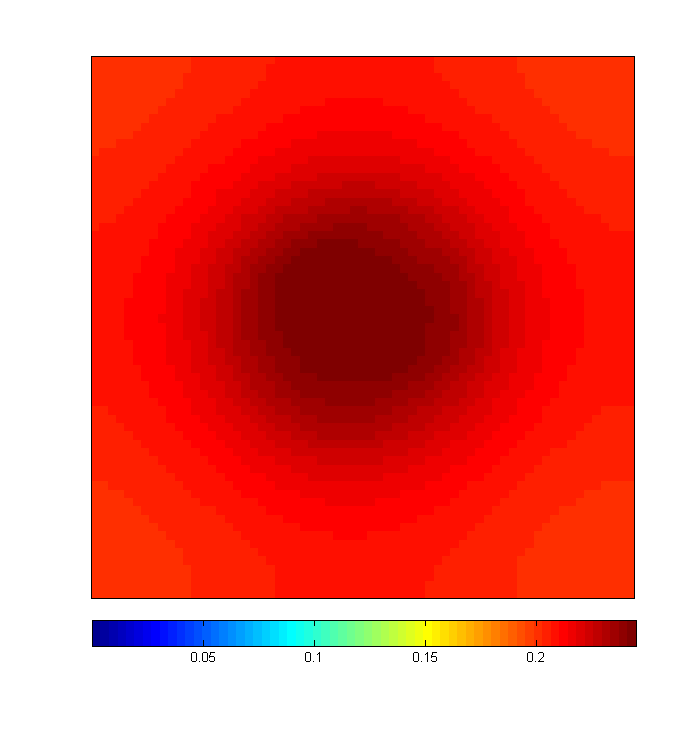
\includegraphics[width=0.20\textwidth]{./figures/O400VEGF solute 072.png} &  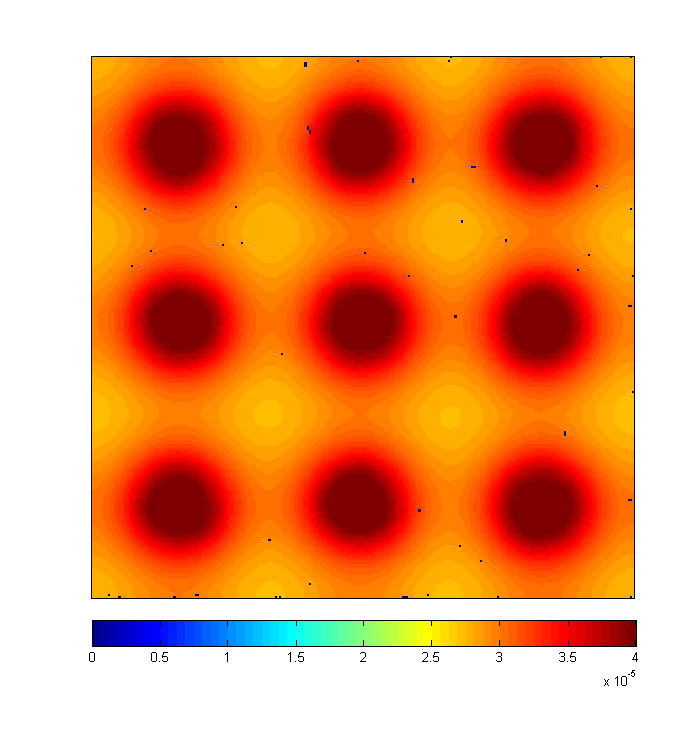
\includegraphics[width=0.20\textwidth]{./figures/C400VEGF solute 072.png} \\
   (c) & (d)
   \end{tabular}
   \end{center}

\caption{(a) Closeup of initial condition of a \SI{400}{\micro\metre} patch (b) Experiment with \SI{400}{\micro\metre}, 3 patches in each side. (c) Closeup of the VEGF distribution after 72 hours, (d) VEGF distribution over whole domain after 72 hours.  }
  \vspace{+1mm}
\label{simulation_examples}
\end{figure}

